\graphicspath{{./fig_Param/}}

%
\section{入力パラメータファイルの記述構文}
%
\subsection{パラメータ記述}
textparserライブラリが扱うパラメータデータベースは,下記のようにノードの階層構造にリーフ(ラベル/値のペア)を格納した構造になっています.パラメータ値のうち,文字列についてはダブルクォーテーションにより囲みます.
textparserライブラリのExamplesディレクトリにパラメータの様々な記述例があるので,参考にしてください.

{
\small 
\begin{program}
  Time_Control {
    Acceleration_Type  = "Time"
    Acceleration       = 1.0
    Dt_Type            = "CFL_Reference_Velocity"
    Delta_T            = 0.2
    Period_Type        = "step"
    Calculation_Period = 20
  }
\end{program}
}


%
\subsection{パラメータファイルの種類と構造}
FFV-Cでは,\textbf{表\ref{tbl:input_files}}に示す二つの入力ファイルを使います.

\begin{table}[htdp]
\caption{パラメータファイル内のセクション}
\begin{center}
\small
\begin{tabular}{ll} \toprule
ファイル & 記述内容\\ \midrule
input.tp & 入力パラメータファイル\\
domain.tp & 計算領域情報ファイル\\ \bottomrule
\end{tabular}
\end{center}
\label{tbl:input_files}
\end{table}


パラメータファイルは,\textbf{表\ref{tbl:param_tag}}に示すセクションがあります.


\begin{table}[htdp]
\caption{パラメータファイル内のセクション}
\begin{center}
\small
\begin{tabular}{ll} \toprule
セクション & パラメータ\\ \midrule
Steer & ソルバー制御\\
Parameter & 計算条件\\
BC\_Table & 境界条件\\
Medium\_Table & 媒質情報\\ \bottomrule
\end{tabular}
\end{center}
\label{tbl:param_tag}
\end{table}


起動時には,次のようにコマンドラインで実行します.
{
\small 
\begin{program}
$ ffvc input.tp domain.tp
\end{program}
}




\pagebreak
%%
\section{計算領域情報ファイル}
計算対象となる領域の情報を与えます.

%
\subsection{DomainInfo}

\begin{indentation}{3zw}{0zw}

{\small
\begin{program}
DomainInfo {
  Global_origin   = (-0.5, -0.5, -0.5   )
  Global_region   = (1.0,  1.0,  1.0    )
  Global_voxel    = (128   , 128   , 128   )
  
  //Global_pitch    = (1.5625e-02, 1.5625e-02, 1.5625e-02)
  //Global_division = (1    , 1    , 1    )

  ActiveSubDomain_File = ""
}
\end{program}
}

計算領域情報については,\textbf{表\ref{tbl:region_info}}に示す計算領域に関するパラメータを指定します.

\begin{table}[htdp]
\caption{DomainInfoセクションにおける計算領域パラメータの指定}
\begin{center}
\small
\begin{tabular}{lll} \toprule
ラベル & 指定内容 & 補足\\ \midrule
Global\_division & 並列計算時の各軸方向の分割数指定 & 任意\\ 
Global\_origin & 計算空間における座標値の最小値 & 必須\\
Global\_pitch & 各軸方向の分割幅 &Global\_voxelと排他,同時指定時に優先\\
Global\_region & 計算領域の大きさ & 必須\\ 
Global\_voxel & 計算空間の各軸方向の分割数 & Global\_pitchと排他\\
ActiveSubDomain\_File & サブドメインの活性・不活性を指定するファイル名 & ファイルがなければブランクを入力\\ \bottomrule
\end{tabular}
\end{center}
\label{tbl:region_info}
\end{table}

\end{indentation}



\pagebreak
%%
\section{入力パラメータファイル}

%
\subsection{Steerセクション}

Steerセクションでは,実行制御パラメータ\index{じっこうせいぎょぱらめーた@実行制御パラメータ}を記述します.\\

%
\subsubsection{Algorithm}

時間積分と\hypertarget{tgt:algorithm}{解法アルゴリズム}の組み合わせを指定するパラメータです.

\begin{indentation}{3zw}{0zw}

{\small
\begin{program}
  Algorithm {
    Flow = "FS_C_EE_D_EE"
    Heat = "C_EE_D_EE"
  }
\end{program}
}

\textbf{表\ref{tbl:alg_flow}}に時間進行法と分離解法の種類の組み合わせを示します.Flowラベルでは流動の支配方程式の時間積分法と解法アルゴリズムの組み合わせを指定します.
%時間二次精度以上を選択した場合には,\verb|Convection_Term|\ref{sec:p_convection}では二次以上の空間スキームしか選択できません.\\

\begin{table}[htdp]
\caption{流動解析のアルゴリズム指定}
\begin{center}
\small
\begin{tabular}{ll} \toprule
ラベル & 時間積分法と解法の組み合わせ\\ \midrule
FS\_C\_EE\_D\_EE & Fractional Step法 + 時間一次精度Euler陽解法(対流項と拡散項)\\ \bottomrule
%FS\_C\_RK\_D\_CN & FS法 + 時間二次精度 Runge-Kutta陽解法(対流項)+ Crank-Nicholson陰解法(拡散項)\\
%FS\_C\_RK\_D\_ME & FS法 + 時間二次精度 Runge-Kutta陽解法(対流項)+ Modified-Euler陽解法(拡散項)\\
%FS\_C\_AB\_D\_AB & FS法 + 時間二次精度 Adams-Bashforth陽解法(対流項と拡散項)\\ \bottomrule
\end{tabular}
\end{center}
\label{tbl:alg_flow}
\end{table}

温度解析の場合には,Heatラベルで温度輸送方程式の時間進行法と解法アルゴリズムの組み合わせを\textbf{表\ref{tbl:alg_heat}}に示します.\\

\begin{table}[htdp]
\caption{温度解析のアルゴリズム指定}
\begin{center}
\small
\begin{tabular}{ll} \toprule
ラベル & 時間積分法と解法の組み合わせ\\ \midrule
C\_EE\_D\_EE & 時間一次精度 Euler陽解法(対流項と拡散項)\\
C\_EE\_D\_EI & 時間一次精度 Euler陽解法(対流項)+ Euler陰解法(拡散項)\\ \bottomrule
%C\_AB\_D\_AB & 時間二次精度 Adams-Bashforth陽解法(対流項と拡散項)\\ \bottomrule
\end{tabular}
\end{center}
\label{tbl:alg_heat}
\end{table}
\end{indentation}



%%%
\pagebreak
\subsubsection{Average\_Option}

\hypertarget{tgt:average_option}{時間平均操作}に関するパラメータを指定します.

\begin{indentation}{3zw}{0zw}

{\small
\begin{program}
  Average_option {
    Operation  = "Off"
    Start_Type = "Time"
    Start      = 500.0
  }
\end{program}
}

\textbf{表\ref{tbl:averaging}}に物理量の時間平均操作\index{じかんへいきんそうさ@時間平均操作}を指定するパラメータを示します.
FFV-Cソルバーは非定常解析を行いますので,流れの挙動が準定常状態になったところで時間平均操作を開始し,十分な長さで時間平均操作が行われた速度場や温度場を定常解\index{ていじょうかい@定常解}とみなします.
時間平均操作の開始時刻はStartで指定し,この開始時刻以降,毎ステップごとに時間平均操作を行います.
平均操作の開始時刻は,Start\_Typeで指定する方法に依存し,
Timeを指定した場合にはUnit\_of\_Input\_Parameterの次元に従います.
つまり,\hyperlink{tgt:unit}{DIMENSIONAL}の場合には有次元時刻で時間平均操作の開始時刻を指定することになります.

時間平均場の出力タイミングは,\hyperlink{tgt:fileio}{File\_IO}のAveraged\_Intervalで指定します.


\begin{table}[htdp]
\caption{Average\_Optionのパラメータ}
\begin{center}
\small
\begin{tabular}{ll} \toprule
ラベル & 指定パラメータ\\ \midrule
Operation & On $|$ Off\\
Start\_Type & 開始時刻の指定 (Step $|$ Time)\\
Start & 時間平均操作の開始時刻\\ \bottomrule
\end{tabular}
\end{center}
\label{tbl:averaging}
\end{table}

\end{indentation}



%%%
\pagebreak
\subsubsection{Check\_Parameter}

入力パラメータの初期化処理時の\hypertarget{tgt:check_parameter}{整合性のチェック}を行い,初期設定後にソルバーを停止します.

\begin{indentation}{3zw}{0zw}

{\small
\begin{program}
  Check_Parameter = "Off"
\end{program}
}

Check\_Parameter=\lq\lq On\rq\rq でチェックが有効な場合,FFV-Cを起動してパラメータを読み込み,前処理が終了した段階で強制終了します.
このとき,初期設定パラメータの内容がconditions.txtに書き出されているので,パラメータのチェックができます.
また,初期条件を与えたフィールドファイルが出力されるので,初期条件のチェックが可能です.

\end{indentation}



%%%
\pagebreak
\subsubsection{Convection\_Term}

\hypertarget{tgt:convection_term}{対流項のスキーム}に関するパラメータを指定します.

\begin{indentation}{3zw}{0zw}

{\small
\begin{program}
  Convection_Term {
    Scheme  = "O3_MUSCL"
    Limiter = "minmod"
  }
\end{program}
}

SchemeとLimiterのパラメータを\textbf{表\ref{tbl:scheme limiter}}に示します.Limiterは制限関数\index{せいげんかんすう@制限関数}の種類を示し,Schemeが\verb|O3_MUSCL|の場合のみ有効となります.
非圧縮流れのように物理量の変化が連続的な場合には不要の場合もあります.
ファイル出力時のオプションでガイドセル出力\hyperlink{tgt:fileio}{Guide\_Out}=\lq\lq with\rq\rq を指定している場合には,対流項スキームによってステンシル\index{ステンシル}が変化するので,ガイドセル\index{ガイドセル}の値も異なります.

\begin{table}[htdp]
\small
\caption{SchemeとLimiterのパラメータ}
\begin{minipage}{.6\textwidth}
\begin{center}
\begin{tabular}{llc} \toprule
ラベル& 指定スキーム & 出力ガイドセルサイズ\\ \midrule
O1\_Upwind & 一次精度風上スキーム & 1\\
O2\_Central & 二次精度中心スキーム & 1\\
O3\_MUSCL & 三次精度MUSCLスキーム & 2\\ \bottomrule
\end{tabular}
\end{center}
\end{minipage} \hfill
\begin{minipage}{.38\textwidth}
\begin{center}
\begin{tabular}{ll} \toprule
ラベル & 制限関数\\ \midrule
Minmod & minmod型\\
No\_Limiter & | \\ \bottomrule
\end{tabular}
\end{center}
\end{minipage}
\label{tbl:scheme limiter}
\end{table}

\end{indentation}



%%%
\pagebreak
\subsubsection{Derived\_Variable}

\hypertarget{tgt:derived_variable}{派生変数}(基本変数から計算される変数)の生成を指定します.

\begin{indentation}{3zw}{0zw}

{\small
\begin{program}
  Derived_Variable {
    Total_Pressure       = "Off"
    Helicity             = "Off"
    Vorticity            = "Off"
    2nd_Invariant_of_VGT = "Off"
  }
\end{program}
}

\textbf{表\ref{tbl:derived vars}}に示す各変数は,on/offのスイッチ指定により有効・無効になり,\hyperlink{tgt:fileio}{File\_IO}セクションのInstant\_Intervalで指定するタイミングでファイルに出力されます.

\begin{table}[htdp]
\caption{派生変数の指定}
\begin{center}
\small
\begin{tabular}{ll}\toprule
ラベル & 生成する派生変数\\ \midrule
Total\_Pressure & 全圧\\
Vorticity & 渦度ベクトル\\
Helicity & ヘリシティ\\
2nd\_Invariant\_of\_VGT & 速度勾配テンソルの第二不変量\\ \bottomrule
\end{tabular}
\end{center}
\label{tbl:derived vars}
\end{table}

%
\paragraph{全圧(総圧)}
全圧の計算を指定した場合には,\verb|tp*.sph|のファイル名でファイルが出力されます\footnote{ワイルドカード*には,ステップ数や並列計算時にはランク番号が入ります}.


全圧は次式で定義され,単位体積あたりのエネルギーを表します.

\begin{equation}
\frac{1}{2} {u^{\prime}}^{2} + \frac{P^{\prime}}{\rho^{\prime}} \qquad [Pa] \sim [J/m^3]
\label{eq:total pressure}
\end{equation}

非圧縮の場合には,

\begin{equation}
{P_{T}}^{\prime} \,=\, \frac{1}{2} \rho^{\prime} {u^{\prime}}^{2} + P^{\prime} \qquad [J/m^3]
\label{eq:total pressure icmp}
\end{equation}

\textbf{式(\ref{eq:total pressure icmp})}は無次元化すると,以下のようになります.

\begin{equation}
P_{T} \,=\, \frac{{P_{T}}^{\prime}}{\rho_{\mathit{0}}^{\prime} {u_{\mathit{0}}^{\prime}}^{2}}
\label{eq:total pressure icmp ND}
\end{equation}

%
\paragraph{渦度ベクトル}
渦度の計算を指定した場合には,\verb|vrt*.sph|のファイル名でファイルが出力されます.

%
\paragraph{ヘリシティ}
ヘリシティの計算を指定した場合には,\verb|hty*.sph|のファイル名でファイルが出力されます.
ヘリシティは速度ベクトル$\overrightarrow{u}$と渦度ベクトル$\overrightarrow{\omega}$の内積として定義される量で次式により表せます.

\begin{equation}
H \,=\, \overrightarrow{u} \cdot \overrightarrow{\omega}
\label{eq:helicity}
\end{equation}


%
\paragraph{速度勾配テンソルの第二不変量}
渦構造を可視化するのに利用され,
符号により単純剪断乱流の中の層状渦と管状渦を区別することができます\cite{tanaka:93:PF}.
\verb|i2vgt*.sph|のファイル名でファイルが出力されます.

\end{indentation}



%%%
\pagebreak
\subsubsection{Example}

\hypertarget{tgt:example}{解くべき問題}を指定します.

\begin{indentation}{3zw}{0zw}

{\small
\begin{program}
  Example = "Performance_Test"
\end{program}
}

\textbf{表\ref{tbl:intrinsic_example}}にFFV-Cソルバーが提供する組み込み例題\index{くみこみれいだい@組み込み例題}の一覧を示します.
組み込み例題で例題固有のパラメータ設定については,Parameter$\to$\hyperlink{tgt:intrinsic_example}{Intrinsic\_Example}をご覧ください.

また,具体的な例題の事例については,例題集をご覧ください.

\begin{table}[htdp]
\caption{Exampleのパラメータ指定}
\begin{center}
\small
\begin{tabular}{ll} \toprule
ラベル & 例題\\ \midrule
Cavity3D & 立方体キャビティ\\
Duct3D & 直方体と円形断面のダクト\\
LDC112 & 辺長比1:1:2の三次元キャビティ\\
Performance\_Test & 性能評価\\
SHC1D & 固体熱伝導\\ \bottomrule
\end{tabular}
\end{center}
\label{tbl:intrinsic_example}
\end{table}

\end{indentation}


%%%
\pagebreak
\subsubsection{File\_IO}

\hypertarget{tgt:fileio}{ファイル入出力モード}を指定します.このセクションでは,入出力ファイルの単位,ガイドセルのモード,ファイル出力モード,並列入出力モード,デバッグ時のファイルなどを指定します.

\begin{indentation}{3zw}{0zw}

{\small
\begin{program}
  File_IO {
    Unit_of_File           = "Non_Dimensional"
    Guide_Out              = "Without"
    Parallel_Input         = "master"
    Parallel_Output        = "master"
    Debug_Divergence       = "Off"
    Instant_Interval_Type  = "step"
    Instant_Interval       = 1000
    Averaged_Interval_Type = "Time"
    Averaged_Interval      = 1000
  }
\end{program}
}

\textbf{表\ref{tbl:file_IO_parameter}}に指定するパラメータの内容を示します.
Unit\_of\_Fileでは入出力する結果ファイル(*.sph)の単位を指定し,有次元か無次元を指定できます.

Guide\_Outラベルで\lq\lq with\rq\rq を指定した場合の出力ガイドセルのサイズは\hyperlink{tgt:convection_term}{Convection\_Term}の項を参照してください.


\begin{table}[htdp]
\caption{ファイル入出力のパラメータ指定}
\begin{center}
\small
\begin{tabular}{llll} \toprule
ラベル & 指定項目 & ラベル & 指定内容 \\ \midrule
Unit\_of\_File & 入出力ファイルの単位 & Dimensional & 有次元\\
& & Non\_Dimensional & 無次元\\ \hline
Guide\_Out & ガイドセル出力モード & with & ガイドセルを一緒に出力\\
& & without & 内部領域のみ出力\\ \hline
Parallel\_Input & ファイル入力 & Master & マスターノードで単一ファイル入出力\\
& & Local  & ローカルノードで分散ファイル入出力 \\ \hline
Parallel\_Output & ファイル出力 & Master & マスターノードで単一ファイル入出力\\
& & Local  & ローカルノードで分散ファイル入出力 \\ \hline
Debug\_divergence & デバッグ時のファイル出力 & On$|$Off & $\nabla \cdot \bm{u}$の出力(無次元値)\\ \hline
Instant\_Interval\_Type & 瞬時値の出力指定形式 & Step & ステップ数指定\\
& & Time & 時間間隔の指定\\
Instant\_Interval & 出力間隔 & | & ステップ数$|$時間間隔\\ \hline
Averaged\_Interval\_Type & 平均値の出力指定形式 & Step & ステップ数指定\\
& & Time & 時間間隔の指定\\
Averaged\_Interval & 出力間隔 & | & ステップ数$|$時間間隔\\\bottomrule
\end{tabular}
\end{center}
\label{tbl:file_IO_parameter}
\end{table}



Parallel\_Input/Outputでは,並列計算時のファイル入出力のモードを指定します.
単一ファイルとして入出力する場合には,Masterを指定します.

デバッグのため,$\nabla \cdot \bm{u}$の値を無次元で出力します.

Intervalのラベルにより,ファイル出力間隔を指定します.
対象となる出力ファイルに対して,時刻またはステップ数によりファイル出力間隔を指定できます.
Instant\_Interval\_TypeあるいはAveraged\_Interval\_Typeが\lq\lq time\rq\rq の場合,時刻の単位は\hyperlink{tgt:unit}{Unit\_of\_Input\_Parameter}で指定したモードに従います.
\end{indentation}





%%%
\pagebreak
\subsubsection{Iteration}

圧力のポアソン方程式や陰解法のように,得られる線形システムの係数行列が大型疎行列となる場合には反復解法\index{はんぷくかいほう@反復解法}を用います.
ここでは流れと温度解析について,\hypertarget{tgt:iteration}{反復法のパラメータを指定}します.

\begin{indentation}{3zw}{0zw}

{\small
\begin{program}
  Iteration {
    Flow {
      Poisson {
        Iteration     = 20
        Epsilon       = 1.0e-3
        Omega         = 1.2
        Norm          = "v_div_max"
        Linear_Solver = "SOR"
        Comm_mode     = "sync"
      }
    }
    Heat {
      Euler_Implicit {
        Iteration     = 30
        Epsilon       = 1.0e-2
        Omega         = 1.2
        Norm          = "T_Res_L2_Absolute"
        Linear_Solver = "SOR"
        Comm_mode     = "async"
      }     
    }     
  }
\end{program}
}

反復法を用いる場合は,\hyperlink{tgt:algorithm}{Algorithm}セクションで反復法を含む解法を指定します.
第2レベルで指定するElem\_nameのラベルは,指定するアルゴリズムに応じて異なり,
\textbf{表\ref{tbl:itr_flow_algo}}に指定アルゴリズムと指定ラベルの関係を示します.
%2nd\_Poissonは二次精度Runge-Kutta法の場合の2nd stepの圧力反復の収束条件を意味します.

\textbf{表\ref{tbl:flow_itr}}には,流動解析の反復解法の指定パラメータを示します.
また,指定可能な収束判定ノルムの種類を\textbf{表\ref{tbl:norm-type}}に示します.


\textbf{表\ref{tbl:LS}}に選択できる反復解法を示します.
表中の△は,並列処理時のデータ依存性(再帰干渉)のために,逐次と並列時で異なる収束特性を示すことを意味します.
%SOR2CMAは反復過程でメモリアクセスが連続になるように並べ替えを行うためにオーバーヘッドが生じるので,反復回数が少ない場合には計算速度向上の効果はない.\\

\begin{table}[htdp]
\caption{流動解析のアルゴリズムと指定ラベル}
\begin{center}
\small
\begin{tabular}{ll} \toprule
Algorithm & 必要なラベル\\ \midrule
FS\_C\_EE\_D\_EE & Poisson\\ \bottomrule
%FS\_C\_AB\_D\_AB & Poisson\\ \bottomrule
%FS\_C\_RK\_D\_ME & 1st\_Iteration, 2nd\_Iteration\\
%FS\_C\_RK\_D\_CN & 1st\_Iteration, 2nd\_Iteration\\ \bottomrule
\end{tabular}
\end{center}
\label{tbl:itr_flow_algo}
\end{table}

\begin{table}[htdp]
\caption{反復条件の指定}
\begin{center}
\small
\begin{tabular}{ll} \toprule
ラベル & 指定内容\\ \midrule
Iteration & 最大反復回数\\
Epsilon & 収束閾値\\
Omega & 加速(緩和)係数\\
Norm & 収束ノルムの種類\\ 
Linear\_Solver & 反復法の指定\\ \hline
Comm\_Mode & 袖通信のモード\\
 & "Sync" 同期通信モード\\
 & "Async" 非同期通信モード\\ \bottomrule
\end{tabular}
\end{center}
\label{tbl:flow_itr}
\end{table}

\begin{table}[htdp]
\caption{流動計算における圧力反復のノルムの指定}
\begin{center}
\small
\begin{tabular}{lll} \toprule
ラベル & 収束判定基準 & 履歴出力のラベル\\ \midrule
V\_Div\_Max & 発散の最大値 $max\left|div\,\bm{u}\right|$ & V\_Div\_Max\\
\vspace{2mm}
V\_Div\_Max\_Monitor & 発散の最大値 $max\left|div\,\bm{u}\right|$の値とセル位置を出力する\footnotemark[1] & V\_Div\_Max\\
\vspace{2mm}
V\_Div\_L2 & 発散の自乗和平方根 $\displaystyle \sqrt{ \sum_{i,j,k}^{Max}{{( {div\,\bm{u}} )}^2}}$ & V\_Div\_L2\\
\vspace{2mm}
P\_Res\_L2\_Absolute & 絶対残差のRMS $\displaystyle \sqrt{ \frac{1}{N} \sum_{i,j,k}^{Max} {\|\vec{b}- A \vec{x}\|}_{2} }$ & P\_Res\_L2\_A\\ 
P\_Res\_L2\_Relative & 相対残差のRMS $\displaystyle {\frac{ \sqrt{ \frac{1}{N} \sum_{i,j,k}^{Max}{\|\vec{b}- A \vec{x}\|}_{2}} } {\sum_{i,j,k}^{Max} {\|\vec{b}\|}_{2} }}$ & P\_Res\_L2\_R\\ \bottomrule
\end{tabular}
\end{center}
\label{tbl:norm-type}
\end{table}
\footnotetext[1]{サーチを行うので,実行速度は遅くなる(デバッグ利用).}

\begin{table}[htdp]
\caption{Linear\_Solverのパラメータ指定}
\begin{center}
\small
\begin{tabular}{llc} \toprule
ラベル & 反復解法 & 並列計算への適用\\ \midrule
Jacobi & 緩和Point Jacobi法 & ○\\
SOR & Point SOR法 & △\\
%SOR2CMA & 連続メモリアクセス型の2色SOR法\\
SOR2SMA & ストライドメモリアクセス型の2色SOR法 & ○\\ \bottomrule
\end{tabular}
\end{center}
\label{tbl:LS}
\end{table}


温度計算で反復法を用いる場合は,\hyperlink{tgt:algorithm}{Algorithm}セクションで反復法を含む解法を指定します.

Flow, Heatのラベルは,それぞれ,流れ計算と熱計算のパラメータであることを示します.
\textbf{表\ref{tbl:itr_temp_algo}}に,指定アルゴリズムと指定ラベルの関係を示します.

温度解析の反復解法のパラメータは,\textbf{表\ref{tbl:flow_itr}}と同じです.
収束ノルムのタイプは\textbf{表\ref{tbl:norm-type4temp}}で指定します.

\begin{table}[htdp]
\caption{温度解析のアルゴリズムと指定ラベル}
\begin{center}
\small
\begin{tabular}{ll} \toprule
Algorithm &  必要なラベル\\ \midrule
C\_EE\_D\_EE & | \\
%C\_AB\_D\_AB & なし\\
C\_EE\_D\_EI & Euler\_Implicit\\ \bottomrule
\end{tabular}
\end{center}
\label{tbl:itr_temp_algo}
\end{table}

\begin{table}[htdp]
\caption{温度計算における反復のノルムの指定}
\begin{center}
\small
\begin{tabular}{lll} \toprule
ラベル & 収束判定 & 履歴出力のラベル\\ \midrule
\vspace{2mm}
T\_Res\_L2\_Absolute & 絶対残差のRMS $\displaystyle \sqrt{ \frac{1}{N} \sum_{i,j,k}^{Max} {\|\vec{b}- A \vec{x}\|}_{2} }$ & T\_Res\_L2\_A\\ 
T\_Res\_L2\_Relative & 相対残差のRMS $\displaystyle {\frac{ \sqrt{ \frac{1}{N} \sum_{i,j,k}^{Max}{\|\vec{b}- A \vec{x}\|}_{2}} } {\sum_{i,j,k}^{Max} {\|\vec{b}\|}_{2} }}$ & T\_Res\_L2\_R\\ \bottomrule
\end{tabular}
\end{center}
\label{tbl:norm-type4temp}
\end{table}

\end{indentation}



%%%
\pagebreak
\subsubsection{LES\_Option}

\hypertarget{tgt:les_option}{LES}(Large-Eddy Simulation)のオプションパラメータを指定します\footnote{\today 現時点で機能未実装.}.

\begin{indentation}{3zw}{0zw}

{\small
\begin{program}
  LES_Option {
    LES_Calculation = "Off"
  }
\end{program}
}

指定できるLESのモデルを\textbf{表\ref{tbl:LES_model}}に示します.

\begin{table}[htdp]
\caption{LESのモデル指定}
\begin{center}
\small
\begin{tabular}{ll} \toprule
ラベル & モデル\\ \midrule
Smagorinsky & 標準スマゴリンスキーモデル\\ \bottomrule
%Low\_Reynolds & 低レイノルズ数型モデル\\
%Dynamic & ダイナミックモデル\\ \bottomrule
\end{tabular}
\end{center}
\label{tbl:LES_model}
\end{table}

\end{indentation}



%%%
\pagebreak
\subsubsection{Log}

\hypertarget{tgt:log}{各種履歴}ファイル\index{ふぁいる@ファイル!りれき@履歴---}出力の制御パラメータを指定します.

\begin{indentation}{3zw}{0zw}

{\small
\begin{program}
  Log {
    Unit_of_Log           = "Non_Dimensional"
    Log_Base              = "On"
    Log_Iteration         = "Off"
    Log_Profiling         = "on"
    Log_Wall_Info         = "Off"
    Console_Interval_Type = "Step"
    Console_Interval      = 1
    History_Interval_Type = "Step"
    History_Interval      = 1
  }
\end{program}
}

Log\_Baseラベルでは,基本履歴ファイルのon/offを制御します.つまり,標準モニタ出力やコンポーネント情報,領域の流量収支履歴の出力を制御します.

Log\_Iterationラベルは,各タイムステップの反復数,残差の最大値とそのインデクス値などの圧力の反復過程の履歴を出力します.
このラベルを \lq\lq on\rq\rq に指定すると,残差は強制的に\hyperlink{tgt:iteration}{V\_Div\_Max}(発散の最大値)となり,\hyperlink{tgt:iteration}{Interation}ラベルでのノルムの指定は無効になります.反復履歴は他の種類のノルムには対応していません.

Log\_Profilingラベルは,実行時に性能測定のための計時を行い,結果をレポートとして出力することを指定します.
Detailオプションにより,詳細なレポートを出力します.
出力項目の詳細は,\hyperlink{tgt:profile}{性能情報}をご覧ください.

Log\_Wall\_Infoは,\hyperlink{tgt:treatment_of_wall}{壁法則}を用いた場合の種々の情報を出力しますが,試験的なものです.

Intervalのラベルにより,ファイル出力間隔を指定します.
対象となる出力ファイルに対して,時刻またはステップ数によりファイル出力間隔を指定できます.
Console\_Interval\_TypeあるいはHistory\_Interval\_Typeがvalue=\lq\lq time\rq\rq の場合,時刻の単位は\hyperlink{tgt:unit}{Unit\_of\_Input\_Parameter}で指定したモードに従います.

Unit\_of\_Logではログ出力の有次元・無次元を指定します.

\begin{table}[htdp]
\caption{履歴ファイルの出力指定}
\begin{center}
\small
\begin{tabular}{lll} \toprule
ラベル & 指定内容 & ラベル$|$指定内容\\ \midrule
Log\_Base & 標準履歴ファイル & ON $|$ OFF\\
Log\_Iteration & 反復解法の反復履歴 & ON $|$ OFF\\
Log\_Profiling & 実行性能レポートの作成・出力 & ON $|$ OFF\\
Log\_Wall\_Info & 壁面情報履歴 & ON $|$ OFF\\ \hline
Console\_Interval\_Type & 標準出力の出力指定形式 & Step (ステップ数指定)\\
& & Time (時刻指定)\\
Console\_Interval & 出力間隔 & ステップ数 $|$ 時刻\\ \hline
History\_Interval\_Type & 履歴ファイルの出力指定形式 & Step (ステップ数指定)\\
& & Time (時刻指定)\\
History\_Interval & 出力間隔 & ステップ数 $|$ 時刻\\ \hline
Unit\_of\_Log & ログファイル中の記述単位 & Dimensional $|$ Non\_Dimensional\\\bottomrule
\end{tabular}
\end{center}
\label{tbl:log_output}
\end{table}

\end{indentation}





%%%
\pagebreak
\subsubsection{Monitor\_List}

ユーザが指定した物理量を指定した位置で\hypertarget{tgt:monitor_list}{サンプリング}し,ファイルに出力する機能です.
サンプリングして出力する機能は2通りの方法で実装されています.
ここでは,指定した座標点で計算結果をサンプリングし,ファイルに出力する方法について説明します.
詳細は,第\ref{chpt:monitor}章をご覧ください.
もう一つの指定方法は,モデルに与えられたラベルを用いて指定する方法で,これについては\hyperlink{tgt:localboundary}{境界条件}セクションをご覧ください.

\begin{indentation}{3zw}{0zw}

{\small
\begin{program}
  Monitor_List {
    Log                    = "Off"
    Output_File            = "sample.log"
    Output_Mode            = "Gather"
    Unit                   = "Non_Dimensional"
    Sampling_Interval_Type = "step"
    Sampling_Interval      = 100
    Cell_Monitor           = "off"

    list[@] {
      type            = "Line"
      label           = "line1"
      value           = "x"
      Variable        = "Velocity"
      Sampling_Method = "Interpolation"
      Sampling_Mode   = "Fluid"
      Division        = 64
      From            = (-0.5, 0.0, 0.0)
      To              = (0.5, 0.0, 0.0)
    }

    list[@] {
      type            = "Line"
      label           = "line2"
      Variable        = "Velocity"
      Sampling_Method = "Interpolation"
      Sampling_Mode   = "Fluid"
      Division        = 64
      From            = (0.0, 0.0, -0.5)
      To              = (0.0, 0.0, 0.5)
    }
  }
\end{program}
}

指定パラメータを\textbf{表\ref{tbl:monitor list}}に示します.
Monitor\_Listには,点群(point\_set)と線分(line)の2種類の指定方法があります.
それぞれをグループと呼び,point\_setの構成点をsetと定義します.

\begin{table}[htdp]
\caption{モニタリストでの指定パラメータ}
\begin{center}
\small
\begin{tabular}{lll} \toprule
ラベル & 指定ラベル & 指定内容\\ \midrule
Log & On $|$ Off & ログ出力指定\\
Output\_Mode & Gather & マスタープロセスに集約して出力\\
& Distribute & 各プロセス毎に出力\\
Unit & 入力パラメータと出力単位の指定 & Dimensional $|$ Non\_Dimensional\\
Sampling\_Interval\_Type & Step $|$ Time & 出力形式の指定\\
Sampling\_Interval & | & 指定間隔\\ 
Cell\_Monitor & On $|$ Off & モニタ出力指定\\ \hline
Point\_Set & & 点群によりモニタ点を指定する\\
Set & & 点の座標を指定する\\
x,y,z & & 座標\\ \hline
Line & & 線分によりモニタ点を指定する\\
From & & 開始点を指定する\\
To & & 終了点を指定する\\
x,y,z & & 座標\\ \hline
Variable & Velocity & 速度を指定\\
 & Pressure & 圧力\\
 & Temperature & 温度\\
 & Total\_Pressure & 全圧\\
 & Vorticity & 渦度\\ \hline
%Velocity\_average & 速度の平均値\\
%Pressure\_average & 圧力の平均値\\
%Temperature\_average & 温度の平均値\\
%Total\_Pressure\_average & 全圧の平均値\\
Sampling\_Method & Nearest & モニタ指定点を含むセルの値\\
 & Interpolation & 三重線形内挿補間\\
 & Smoothing & 局所平均による平滑化\\ \hline
Sampling\_Mode & All & 全セルを対象とする\\
 & Fluid & 流体セルのみを対象とする\\
 & Solid & 固体セルのみを対象とする\\ \bottomrule
\end{tabular}
\end{center}
\label{tbl:monitor list}
\end{table}

\begin{itemize}
\item モニタ出力機能は,LogラベルでON/OFFを指定します.
\item 出力ファイル名は,Output\_Fileラベルで指定します.
\item 出力モードはOutput\_Modeラベルで指定します.
これは並列計算時のファイル出力方式で,マスターノードに集約してファイル出力する場合にはGatherを指定し,分散ノード毎にファイル出力する場合にはDistributeを指定します.
\item Variableラベルでは,サンプリングする物理量を指定します.
物理量はpoint\_setの例のように複数指定可能です.
\item Sampling\_Methodラベルで指定されるパラメータは,サンプリング方法を指定します.
\item Sampling\_Modeで指定されるパラメータは,サンプリングモードを指定します.
\item ファイル出力間隔は,Sampling\_Intervalで指定し,その指定単位をSampling\_Interval\_Typeで指定します.
\item Unitラベルでは,Monitor\_Listセクションで指定するパラメータの単位と出力するログの単位を指定します.指定パラメータと出力ログの単位は同じになります.
\end{itemize}

\end{indentation}



%%%
\begin{comment}
\pagebreak
\subsubsection{Polygon\_File}
\hypertarget{tgt:poly_file_name}{ポリゴンファイル名}を指定します.

\begin{indentation}{3zw}{0zw}
\small

\hyperlink{tgt:solver_property}{Shape\_Approximation}でDistance\_Infoを指定すると,距離情報を用いたスキームでの計算となります.この場合,ポリゴンファイルが必要となりますが,そのポリゴンファイルを記述したファイル名をこのセクションで指定します.
ポリゴンファイルと\hyperlink{tgt:domaininfo}{DomainInfo}の指定のみで計算をする場合には,\hyperlink{tgt:polygon_class}{IP\_Polygonクラス}を指定します.

\begin{program}
<Elem name="Polygon_File">
  <Param name="File_Name" dtype="string" value="polygon.xml"/>
</Elem>
\end{program}

\end{indentation}
\end{comment}


\pagebreak
\mbox{ }


%%%
\pagebreak
\subsubsection{Reference\_Frame}

\hypertarget{tgt:reference_frame}{観測}の座標系\index{ざひょうけい@座標系}を指定します.

\begin{indentation}{3zw}{0zw}
\small

\begin{program}
  Reference_Frame {
    Reference_Frame_Type = "Stationary"
  }

\end{program}

\normalsize
FFV-Cソルバーでは,\textbf{表\ref{tbl:ref_frame}}に示す選択肢があります.
移動座標系\index{ざひょうけい@座標系!いどう@移動---}を指定する場合には,格子の移動速度の各方向成分(有次元では$[m/s]$)を入力します.
座標系は右手系をとり,各軸x, y, z方向の速度成分をそれぞれu, v, wとします.
静止座標系\index{ざひょうけい@座標系!せいし@静止---}と移動座標系とでは,同じ問題を解く場合でも与える境界条件が異なるので注意します.

\begin{table}[htdp]
\caption{Reference\_Frameの指定}
\begin{center}
\small
\begin{tabular}{lll} \toprule
ラベル & 指定パラメータ & 参照座標系\\ \midrule
Stationary & | & 静止座標系\\
Translational & $u,\,v,\,w$ & 並進運動する移動座標系\\ \bottomrule
%Rotational & $u,\,v,\,w$ & 回転運動する座標系\\ \bottomrule
\end{tabular}
\end{center}
\label{tbl:ref_frame}
\end{table}

\end{indentation}



%%%
\pagebreak
\subsubsection{Start\_Condition}

計算の\hypertarget{tgt:start_condition}{スタート条件}を指定します.

\begin{indentation}{3zw}{0zw}

{\small
\begin{program}
  Start_Condition {
    Start_Type         = "initial"
    Restart_step       = 200
    Prefix_of_Pressure = "prs_"
    Prefix_of_Velocity = "vel_"
    dfi_file_pressure  = "prs_64_id000000.dfi"
    dfi_file_velocity  = "vel_64_id000000.dfi"
    Initial_State {
      Density     = 1.0
      Pressure    = 0.0
      Temperature = 20.0
      Velocity    = (0.0, 0.0, 0.0)
    }
  }
\end{program}
}

\textbf{表\ref{tbl:start}}に選択肢を示します.


\begin{table}[htdp]
\caption{Start\_Conditionのパラメータ指定}
\begin{center}
\small
\begin{tabular}{lll} \toprule
ラベル & スタートの種類 & \\ \midrule
Start\_Type & スタートの種類 & \\
 & Initial & 時刻ゼロからの初期スタート\\
 & Restart & リスタート\\ \hline
Restart\_Step & & リスタートのステップ数を指定\\ \hline
dfi\_file\_pressure & & 粗格子からリスタートする場合の圧力ファイル名を指定\\
dfi\_file\_velocity & & 粗格子からリスタートする場合の速度ファイル名を指定\\ \hline
Initial\_State & 初期条件を指定 & \\
Density & & 密度\\
Pressure & & 圧力\\
Velocity & & 速度ベクトル\\ \bottomrule
\end{tabular}
\end{center}
\label{tbl:start}
\end{table}

\hypertarget{tgt:initial_state}{物理変数}の初期値\index{しょきち@初期値}を指定します.

記述する初期値は有次元量で指定しますが,Solver\_Propertyセクションで\hyperlink{tgt:solver_property}{Kind\_of\_Solver}=\lq\lq Flow\_Only\rq\rq を指定した場合のみ,無次元での指定も可能です.
圧力値は,\hyperlink{tgt:unit}{Unit}で指定する圧力の単位に従います.
各変数の無次元化は以下のようになり,添え字の0は代表値または基準値を意味します.

\begin{equation}
\left.
\begin{array}{l}
\vspace{2mm}
\displaystyle{ \rho \,=\, \frac{\rho^{\prime}}{\rho_{0}^{\prime}} } \\
\vspace{2mm}
\displaystyle{ p \,=\, \frac{p^{\prime}-p_{0}^{\prime}}{\rho_{0}^{\prime}\,{u_{0}^{\prime}}^{2}} } \\
\vspace{2mm}
\displaystyle{ u_{i} \,=\, \frac{u_{i}^{\prime}}{u_0^{\prime}} } \\
\vspace{2mm}
\displaystyle{ \theta \,=\, \frac{\theta^{\prime}-\theta_{0}^{\prime}}{\Delta \theta^{\prime}} } 
\end{array} \qquad \right \}
\end{equation}

\end{indentation}



%%%
\pagebreak
\subsubsection{Solver\_Property}

ソルバーの\hypertarget{tgt:solver_property}{基本的なパラメータ}を設定します.ここでは,支配方程式の型の選択,浮力モード,形状近似などのパラメータを指定します.

\begin{indentation}{3zw}{0zw}

{\small
\begin{program}
  Solver_Property {
    Basic_Equation      = "Incompressible"
    Buoyancy            = "No_Buoyancy"
    Kind_of_Solver      = "Flow_Only"
    PDE_type            = "Navier_Stokes"
    Shape_Approximation = "Binary"
    Time_Variation      = "Unsteady"
    Pressure_Shift      = "off"
  }
\end{program}
}

Basic\_Equationには,\textbf{表\ref{tbl:basic_eq}}に示す支配方程式の形式を示します.

\begin{table}[htdp]
\caption{Basic\_Equationのパラメータ指定}
\begin{center}
\small
\begin{tabular}{ll} \toprule
ラベル & 支配方程式\\ \midrule
%Compressible & 圧縮性\\ \bottomrule
Incompressible & 非圧縮性\\ \bottomrule
%Limited\_Compressibility & 微小圧縮性\\ \bottomrule
\end{tabular}
\end{center}
\label{tbl:basic_eq}
\end{table}

PDE\_typeで指定する方程式の型は,\textbf{表\ref{tbl:PDE type}}から選択します.
デフォルトでNavier Stokesで,Eulerはテスト用のパラメータです.

\begin{table}[htdp]
\caption{PDE\_typeのパラメータ指定}
\begin{center}
\small
\begin{tabular}{ll} \toprule
ラベル & PDEの型\\ \midrule
Navier-Stokes & Navier-Stokes方程式\\
Euler & Euler方程式\\ \bottomrule
\end{tabular}
\end{center}
\label{tbl:PDE type}
\end{table}

Kind\_of\_Solverには,\textbf{表\ref{tbl:kos}}に計算する問題の熱流動現象の分類(熱流動タイプ\index{ねつりゅうどうたいぷ@熱流動タイプ})を示します.
熱伝導方程式を指定している場合(Kind\_Of\_Solver=\lq\lq SOLID\_CONDUCTION\rq\rq )には,Heat Conduction Equationと表示されます.
また,Buoyancyの指定は,Kind\_of\_Solverが必要とする場合にのみ有効になります.

\begin{table}[htdp]
\caption{熱対流計算とKind\_Of\_SolverおよびBuoyancyの関係}
\begin{center}
\small
\begin{tabular}{lll} \toprule
支配方程式 & Kind\_of\_Solver & Buoyancy\\ \midrule
純強制対流 & Flow\_Only & |\\
強制熱対流(浮力なし)& Thermal\_Flow & No\_Buoyancy\\
強制熱対流(浮力あり)& Thermal\_Flow & Boussinesq\\
%& & Low\_Mach\\
自然対流 & Thermal\_Flow\_Natural & Boussinesq\\
%& & Low\_Mach\\
固体熱伝導 & Solid\_Conduction & |\\ \bottomrule
%共役熱移動 & Conjugate\_Heat\_Transfer & Boussinesq\\ 
%& & Low\_Mach\\ \bottomrule
\end{tabular}
\end{center}
\label{tbl:kos}
\end{table}

\pagebreak
Shape\_Approximationラベルには,\textbf{表\ref{tbl:ShapeApprox}}に示す解析モデルの形状近似モードを指定します.

\begin{table}[htdp]
\caption{形状近似モードの指定}
\begin{center}
\small
\begin{tabular}{ll} \toprule
ラベル & 形状近似\\ \midrule
Binary & バイナリボクセル近似\\
Distance\_Info & 距離情報近似\\ \bottomrule
%Implicit\_Function & 陰関数近似\\ 
%Level\_Set & レベルセット関数近似\\
%Volume\_Fraction & 体積率近似\\ \bottomrule
\end{tabular}
\end{center}
\label{tbl:ShapeApprox}
\end{table}

Time\_Variationラベルでは,\textbf{表\ref{tbl:steady}}に示すパラメータにより,解析する現象として定常あるいは非定常を指定します.
\begin{table}[htdp]
\caption{非定常モードの指定}
\begin{center}
\small
\begin{tabular}{ll} \toprule
ラベル & モードの指定\\ \midrule
Steady & 定常\\
Unsteady & 非定常\\ \bottomrule
\end{tabular}
\end{center}
\label{tbl:steady}
\end{table}


Pressure\_Shiftラベルは,圧力値をシフトします.
指定方向の計算領域の最外側セルにおける空間平均値を全計算空間から差し引き,指定面の圧力をゼロとします.

\begin{table}[htdp]
\caption{Pressure\_Shiftの指定}
\begin{center}
\small
\begin{tabular}{ll} \toprule
指定値 & \\ \midrule
off & 圧力値をシフトしない\\
X\_Minus & X-面\\
X\_Plus & X+面\\
Y\_Minus & Y-面\\
Y\_Plus & Y+面\\
Z\_Minus & Z-面\\
Z\_Plus & Z+面\\ \bottomrule
\end{tabular}
\end{center}
\label{tbl:steady}
\end{table}


\end{indentation}



%%%
\pagebreak
\subsubsection{Time\_Control}

\hypertarget{tgt:time_control}{時刻設定}に関するパラメータを指定します.

\begin{indentation}{3zw}{0zw}

{\small
\begin{program}
  Time_Control {
    Acceleration_Type  = "Time"
    Acceleration       = 1.0
    Dt_Type            = "CFL_Reference_Velocity"
    Delta_T            = 0.2
    Period_Type        = "step"
    Calculation_Period = 20
  }
\end{program}
}

%
\paragraph{Acceleration}
Accelerationラベルは,イニシャルスタート\index{イニシャルスタート}の場合にのみ有効なパラメータで,一定速度になるまでの時間を指定します.
Acceleration\_Typeで指定する時間の単位を指定します.
指定単位がTimeの場合,加速時間の値はUnitセクションの\hyperlink{tgt:unit}{Unit\_of\_Input\_Parameter}で指定するモード(Dimensional/Non\_Dimensional)に従います.計算初期の急加速による発散を防ぐため,格子の移動速度や指定流速をゼロから徐々に加速し,指定の値に漸近させる目的で利用します.
加速時間を長くとると流れの発達に時間がかかるので,発散しない程度の時間を設定します.
加速時間$t_0$は計算領域を通過する時間程度が適切で,$t_0\,=\,L/u_0$を参考にします.ここで$L$は領域長さで$u_0$は代表速度とします.
値として0.0を指定すると急加速になります.
加速時間中は,参照速度$u_{Ref}$に対して次式の加速曲線を与え,\textbf{図\ref{fig:accel_velocity}}のように滑らかに一定速度に漸近させます.

\begin{equation}
u_{Ref}\,=\,
\begin{cases}
\, \displaystyle {\frac{1}{2}}\left(1-\cos \left( \frac{t}{t_{0}}\pi \right) \right) & \quad (t < t_{0})\\
\, 1.0 & \quad (t \geqq t_{0})\\
\end{cases}
\label{eq:Ref_velocity_eq}
\end{equation}

\begin{figure}[htdp]
\begin{center}
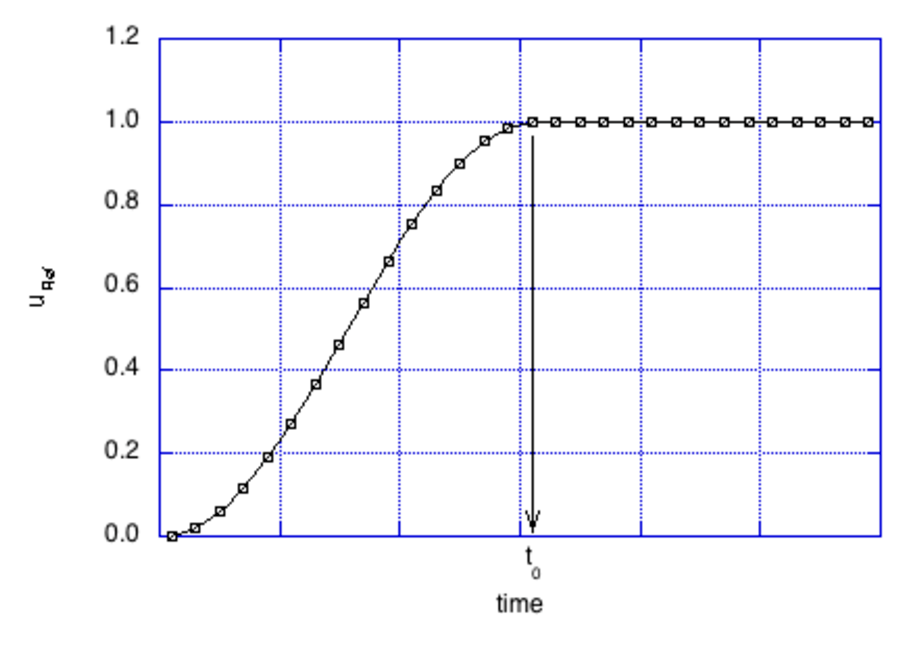
\includegraphics[width=7cm,clip]{accel_Velocity.eps}
\end{center}
\caption{加速中の速度プロファイル}
\label{fig:accel_velocity}
\end{figure}

%
\paragraph{時間積分幅$\Delta{t}$の指定}
\textbf{表\ref{tbl:delta t inc}}に時間積分幅\index{じかんせきぶんはば@時間積分幅}$\Delta{t}$の指定方法を示します.
拡散数\index{かくさんすう@拡散数}$D$は一次元の拡散方程式の場合$D=\alpha \Delta t \slash h^2$で与えられます.$\alpha$は拡散係数で,Navier-Stokes方程式の場合$1/Re$,温度の輸送方程式の場合には$1/Pe$となります.安定性解析から$D<1 \slash 2$であることが要請されます.多次元の場合には,$d_m$を次元数として$\delta t<h^2 \slash (2d_m \alpha)$となります.

Delta\_tにはCFL数\index{CFL},または$\Delta t$を記述します.
時間積分幅の選択は,ソルバの種類を示すKind\_of\_Solverパラメータと関連があり,Solid\_Conductionの場合にはDt\_Directのみ選択できます.

\begin{table}[htdp]
\caption{Time\_Incrementのパラメータ指定}
\begin{center}
\small
\begin{tabular}{lll} \toprule
Dt\_Type & 時間積分幅の決定方法 & Delta\_tへの指定数値\\ \midrule
Direct & $\Delta t$を直接指定する & $\Delta t$\\
%CFL\_DFN\_MaxV & CFL\_MaxVと拡散数により制限される$\Delta t$の値の小さい方を選択\\
%CFL\_DFN\_RefV & CFL\_RefVと拡散数により制限される$\Delta t$の値の小さい方を選択\\
%CFL\_MaxV & CFL数を指定し,瞬時値の最大流速から$\Delta t$を決定 & CFL数\\
CFL\_Reference\_Velocity & CFL数を指定し,代表流速から$\Delta t$を決定 & CFL数\\
Diffusion & 拡散数から$\Delta t$を決定 & |\\
CFL\_Diffusion\_Reference\_Velocity & 代表流速に対するCFL数と拡散数から$\Delta t$を決定 & CFL数\\
%CFL\_MaxV\_CP & CFL数を指定し,音速を考慮した瞬時値の最大流速から$\Delta t$を決定 & CFL数\\
 \bottomrule
\end{tabular}
\end{center}
\label{tbl:delta t inc}
\end{table}



%%%
\pagebreak
\paragraph{計算時間の指定}
Period\_Typeで計算する時間の記述単位を指定します.
計算時間を時間で指定する場合,時間の単位は\hyperlink{tgt:unit}{Unit\_of\_Input\_Parameter}のモードに従います.
指定された単位の数値をCalculation\_Periodで指定します.

\end{indentation}



%%%
\pagebreak
\subsubsection{Treatment\_of\_Wall}

\hypertarget{tgt:treatment_of_wall}{壁面の扱い}について指定します.本パラメータは実験的実装です.

\begin{indentation}{3zw}{0zw}

{\small
\begin{program}
  Treatment_of_Wall {
    Pressure_Gradient = "Grad_Zero"
    Velocity_Profile  = "No_Slip"
  }
\end{program}
}

各パラメータの意味について,\textbf{表\ref{tbl:wall_treatment}}に示します.
圧力勾配は法線方向の圧力勾配ゼロとNavier-Stokes方程式の圧力項を評価する2つの扱いが選択できます\footnote{現時点では,圧力勾配ゼロのみが選択できます.}.
速度プロファイルについては,滑りなし条件と壁関数を用いた近似が選択できます.壁関数は対数則が実装されています.詳細はCBCソルバークラス説明書をご覧ください\footnote{\today 未リリース.}.

\begin{table}[htdp]
\caption{壁面条件の指定}
\begin{center}
\small
\begin{tabular}{lll} \toprule
ラベル & パラメータの値 & 説明\\ \midrule
Pressure\_Gradient & Grad\_Zero & 圧力勾配ゼロ\\
 & Grad\_NS & Navier-Stokes方程式から計算する\\ \hline
Velocity\_Profile  & No\_Slip & 滑りなし壁面条件\\
 & Slip & 滑り壁条件\\
 & Law\_of\_Wall & 壁法則\\ \bottomrule
\end{tabular}
\end{center}
\label{tbl:wall_treatment}
\end{table}

\end{indentation}



%%%
\pagebreak
\subsubsection{Unit}

入力ファイルと出力ファイルで用いる\hypertarget{tgt:unit}{単位を指定}します.

\begin{indentation}{3zw}{0zw}

{\small
\begin{program}
  Unit {
    Unit_of_Input_Parameter = "Non_Dimensional"
    Pressure                = "Gauge"
    Temperature             = "Celsius"
  }
\end{program}
}

各ラベルは,\textbf{表\ref{tbl:param_unit}}に示す単位の指定に用いられます.
有次元のファイル出力時には,圧力単位としてゲージ圧(Gauge Pressure)と絶対圧力(Absolute Pressure)が選択できます.
\textbf{式(\ref{eq:gauge pressure})}に示すゲージ圧を\textbf{式(\ref{eq:ND gauge})}により無次元化する場合に,基準圧として$p_0^\prime\,=\,1.0325\times 10^5$ [Pa]を用い,動圧が$10^0 \sim 10^3$程度とすると,$p \sim \mathrm{O}(1)$程度となるので,単精度計算では4桁程度有効桁が失われる場合もあります.
そのような場合,有次元値のファイル出力単位としてゲージ圧$p_g^\prime$を用います(非圧縮流れの場合には圧力差が意味をもつので,ゲージ圧でもかまいません).
ゲージ圧の基準となる大気圧$p_0^\prime\,$[Pa]は\hyperlink{tgt:reference}{Base\_Pressure}で指定します.
圧力単位の指定は,履歴ファイルのモニタ値にも適用されます.

\begin{equation}
p_g^\prime \,=\, p^\prime \,-\, p_0^\prime
\label{eq:gauge pressure}
\end{equation}

\begin{equation}
p \,=\, \frac{p_g^\prime}{\rho^\prime {u_0^\prime}^2}
\label{eq:ND gauge}
\end{equation}

\begin{table}[htdp]
\caption{単位の指定}
\begin{center}
\small
\begin{tabular}{lll} \toprule
ラベル & 指定パラメータ & 説明\\ \midrule
Unit\_of\_Input\_Parameter & Dimensional or Non\_Dimensional & 入力パラメータファイルの単位を指定します(*1)\\
Pressure & Gauge or Absolute & 入力パラメータの単位が有次元のときに有効となります\\
Temperature & Celsius or Kelvin & 入力パラメータの単位が有次元のときに有効となります\\\bottomrule
\end{tabular}
\end{center}
\label{tbl:param_unit}
\end{table}

\end{indentation}



%%%
\pagebreak
\subsubsection{Version\_Info}

FFV-CソルバーとFlowBaseクラスの\hypertarget{tgt:version}{バージョン番号}を指定します.
異なる番号を指定している場合には,修正すべきバージョン番号が表示されるので入力パラメータファイルを変更します.

\begin{indentation}{3zw}{0zw}
\small
\begin{program}
  Version_Info {
    FFV       = 40
    Flow_Base = 90
  }
\end{program}

\end{indentation}



%%% 隠しパラメータ
\begin{comment}
\subsubsection{Variable\_Range}

温度計算を実施する場合に,変数値を無次元値で[0,1]の範囲に\hypertarget{tgt:variable_range}{制限}することを指定します.

\begin{indentation}{3zw}{0zw}
\small

\begin{program}
<Param name="Variable_Range"     dtype="STRING" value="normal" />
\end{program}

\normalsize
温度の値に制限を課す場合に\textbf{表\ref{tbl:var_range}}に示すパラメータを使用します.保存則を満たさなくなるため,影響を考慮して利用してください.

\begin{table}[htdp]
\small
\caption{Variable\_Rangeのパラメータ指定}
\begin{center}
\begin{tabular}{ll} \toprule
ラベル & モード\\ \midrule
cutoff & 値を無次元で[0, 1]に制限します\\
normal & 制限しません\\ \bottomrule
\end{tabular}
\end{center}
\label{tbl:var_range}
\end{table}

\end{indentation}
\end{comment}


%%%
\pagebreak
\subsection{Parameterセクション}

パラメータセクションでは,FFV-Cソルバーの実行に必要な物理パラメータ\index{ぶつりぱらめーた@物理パラメータ}を記述します.


%%%
\subsubsection{Init\_Temp\_of\_Medium}
温度計算の場合に,割り当てた\hypertarget{tgt:initial_temp}{媒質}に対して初期温度を設定します.


{\small
\begin{program}
  Init_Temp_of_Medium {
    Medium[@] {
      label       = "air"
      Temperature = 20.0
    }
    Medium[@] {
      label       = "Fe"
      Temperature = 50.0
    }
  }
\end{program}
}



%%%
\pagebreak
\subsubsection{Intrinsic\_Example}

\hypertarget{tgt:intrinsic_example}{組み込み}例題\index{くみこみれいだい@組み込み例題}に固有のパラメータを指定します.

\begin{indentation}{3zw}{0zw}
\small

\begin{program}
  Intrinsic_Example {
    fluid_medium = "air"
    solid_medium = "fe"
  }
\end{program}

\normalsize
指定可能なパラメータは,\textbf{表\ref{tbl:intrinsic_parameter}}に示すように各\hyperlink{tgt:example}{組み込み例題}ごとに異なります.

\begin{table}[htdp]
\caption{Intrinsic\_Exampleセクションで指定できるパラメータ}
\begin{center}
\small
\begin{tabular}{llll} \toprule
組み込み例題 & 指定パラメータラベル & dtype & 指定値\\ \midrule
Duct3D & Shape     & STRING & Circular, Rectangular\\
       & Diameter  & REAL   & 断面径 [m]\\
       & Direction & STRING & X\_minus $|$ X\_plus $|$ Y\_minus $|$ Y\_plus $|$ Z\_minus $|$ Z\_plus\\
       & Driver    & REAL   & ドライバ部分の長さ [m]\\ \bottomrule
\end{tabular}
\end{center}
\label{tbl:intrinsic_parameter}
\end{table}

\end{indentation}



%%%
\pagebreak
\subsubsection{Reference}

解析に用いる無次元化の\hypertarget{tgt:reference}{基準量},あるいは無次元パラメータを指定します.

\begin{indentation}{3zw}{0zw}

{\small
\begin{program}
  Reference {
    Length        = 1.0
    Velocity      = 1.0
    Gravity       = 9.8
    Base_Pressure = 0.0
    Reynolds      = 1000.0
    Prandtl       = 0.71
    Base_Medium   = "air"
  }
\end{program}
}

\noindent \textbf{表\ref{tbl:ref_value}}に示すように基準量を必要に応じて記述できます.
無次元パラメータであるReynolds数とPrandtl数は,\hyperlink{tgt:unit}{Unit}の指定が無次元のときのみ指定できます.
Base\_Mediumで指定する名前は,モデル内で使われている必要があります.
固体熱伝導解析の場合には固体のラベルを指定し,それ以外の(熱)流動解析の場合には流体のラベルを指定します.

\begin{table}[htdp]
\caption{Referenceセクションで指定できるパラメータ}
\begin{center}
\small
\begin{tabular}{llll} \toprule
値 & 意味 & 単位\\ \midrule
Length & 代表長さ & $m$ &\\
Velocity & 代表速度 & $m/s$ &\\
Base\_Pressure & 基準圧力 & $Pa$ &\\
Gravity & 重力加速度 & $m^2/s$ &\\
%Grashof & グラショフ数 & |\\
Prandtl & プラントル数 & | & 無次元のときのみ指定\\
%Rayleigh & レイリー数 & |\\
Reynolds & レイノルズ数 & | & 無次元のときのみ指定\\
Base\_Medium & 代表物性値として指定する媒質ラベル & | &\\ \bottomrule
\end{tabular}
\end{center}
\label{tbl:ref_value}
\end{table}

\end{indentation}



%%%
\pagebreak
\subsubsection{Temperature}

\hypertarget{tgt:temperature}{温度計算}を実施する場合の基準量を有次元値で指定します.

\begin{indentation}{3zw}{0zw}

{\small
\begin{program}
  Temperature {
    Base       = 20.0
    Difference = 35.0
  }
\end{program}
}

基準温度(Base)と温度差(Difference)は,非圧縮計算のパッシブスカラーによる温度計算では温度場を特徴づける代表量となります.
単位は\hyperlink{tgt:unit}{Temperature}ラベルで指定します.

\end{indentation}



%%%
\pagebreak
\subsection{Medium\_Tableセクション}

ソルバーで利用する媒質の\hypertarget{tgt:medium_table}{物性値テーブル}を記述します.
ここで記述する媒質の基本リスト\index{きほんりすと@基本リスト!ばいしつの@媒質の---}は,解析に利用される候補です.
媒質は流体と固体が記述でき,\textbf{表\ref{tbl:MTLentry}}により媒質を指定します.

\begin{indentation}{3zw}{0zw}

{\small
\begin{program}
Medium_Table {

  Medium[@] {
    type                 = "Fluid"
    label                = "Air"
    Density              = 1.1763
    Specific_Heat        = 1007
    Thermal_Conductivity = 2.614e-02
    Kinematic_Viscosity  = 15.83e-06
    Viscosity            = 18.62e-06
    Sound_of_Speed       = 340.0
    volume_expansion     = 0.04e-3 
  }

  Medium[@] {
    type                 = "Solid"
    label                = "Fe"
    Density              = 7870.0
    Specific_Heat        = 442.0
    Thermal_Conductivity = 80.3
  }

}
\end{program}
}

\begin{table}[htdp]
\caption{Medium\_Tableに記述するパラメータ}
\begin{center}
\begin{tabular}{ll} \toprule
ラベル & 説明\\ \midrule
Type & Fluid または Solid\\
Label & 媒質名\\ \bottomrule
\end{tabular}
\end{center}
\label{tbl:MTLentry}
\end{table}


各媒質は固体と流体によって記述しなければならない物性値が異なります.
指定できる項目を\textbf{表\ref{tbl:medium_tbl}}に示します.
固体については,密度・比熱・熱伝導率のみの記述となります.
各媒質の情報は,任意に指定するID番号によって管理されます.

\begin{table}[htdp]
\caption{Medium\_Tableにおける物性値の指定}
\begin{minipage}{.45\textwidth}
\begin{center}
\begin{tabular}{lll}\\ \toprule
Fluidのラベル & 説明 & 単位\\ \midrule
Density & 密度 & $kg/m^3$\\
Specific\_Heat & 定圧比熱 & $kJ/(kg K)$\\
Thermal\_Conductivity & 熱伝導率 & $W/(m K)$\\
Kinematic\_Viscosity & 動粘性係数 & $m^2/s$\\
Viscosity & 粘性係数 & $Pa\,s$\\
Sound\_of\_Speed & 音速 & $m/s$\\
Volume\_Expansion & 体膨張率 & $1/K$\\ \bottomrule
\end{tabular}
\end{center}
\end{minipage} \hfill
\begin{minipage}{.45\textwidth}
\begin{center}
\begin{tabular}{lll}\\ \toprule
Solidのラベル & 説明 & 単位\\ \midrule
Density & 密度 & $kg/m^3$\\
Specific\_Heat & 定圧比熱 & $kJ/(kg K)$\\
Thermal\_Conductivity & 熱伝導率 & $W/(m K)$\\ \bottomrule
\end{tabular}
\end{center}
\end{minipage}
\label{tbl:medium_tbl}
\end{table}

\end{indentation}

